% -*- root: ../EstadisticaII.tex -*-

\chapter{Regresión}
El objetivo de la regresión es predecir una/s variable/s en función de la/s otra/s.


\section{Regresión lineal}

Observamos dos variables, X e Y , el objetivo es analizar la relaci´on existente entre ambas, de forma que podamos predecir o aproximar el valor de la variable Y a partir del valor de la variable X.

\begin{itemize}
\item La variable Y se llama variable respuesta.
\item La variable X se llama variable regresora o explicativa.
\end{itemize}

Por ejemplo:
\begin{center}
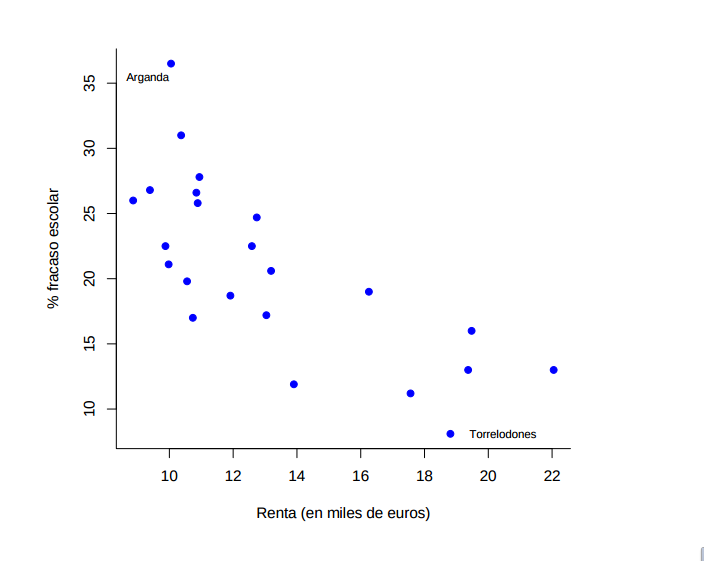
\includegraphics[scale=0.8]{img/RentaVsFracaso.png}
\end{center}

Queremos predecir el fracaso escolar en función de la renta. La variable respuesta es el fracaso escolar, mientras que la variable regresora es la renta. 

\subsection{Regresión lineal simple}

Frecuentemente existe una relación lineal entre las variables. En el caso del fracaso escolar,queremos construir una recta $Y_i = β_0 X_i + β_1\; i=1,...,n$ que minimice el error.

El problema es estimar los parámetros $β_0,β_1$. Una manera de hacer esto es:

\subsubsection{Recta de mínimos cuadrados}

\begin{defn}[Recta de mínimos cuadrados]
Estimando $β_i$ por $\gor{β_i}$ obtenemos: \[\gor{Y_i} = \gor{β}_0 + \gor{β}_1 x_i\]

La reca viene dada por los valores $\gor{β_0} \gor{β_1}$ para los que se minimiza:
\[\sum_{i=1}^n \left[ Y_i - (\gor{β_0} + \gor{β_1}x_i) \right]^2\]
\end{defn}

\begin{example}
\begin{center}
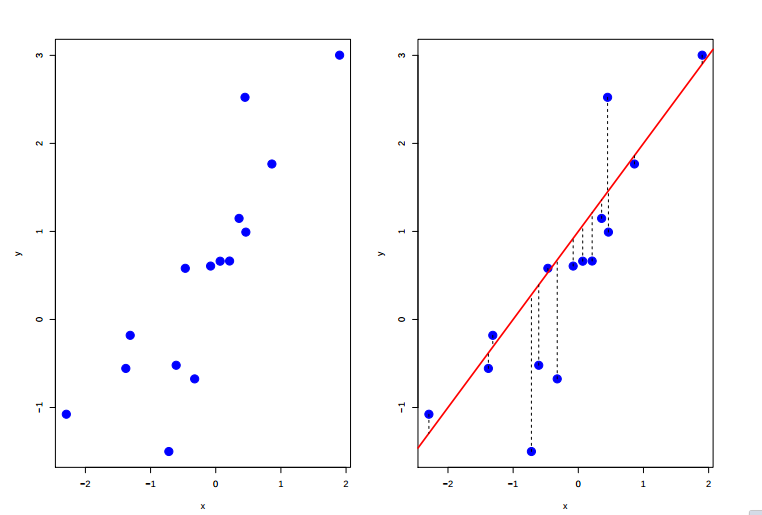
\includegraphics[scale=0.6]{img/ejemploRectaRegresionLineal.png}
\end{center}

\end{example}

\subsection{Regresión lineal múltiple}


\subsection{Estimadores de mínimos cuadrados}
\subsection{Inferencia sobre los parámetros del modelo}
\subsection{Análisis de la varianza}
\subsection{Contrastes de hṕótesis lineales}
\subsection{Modelo unifactorial}